\subsubsection{最大流}

\textbf{判断一条边是否必定满流}

在残量网络中跑一遍Tarjan, 如果某条满流边的两端处于同一SCC中则说明它不一定满流. (因为可以找出包含反向边的环, 增广之后就不满流了.)

\subsubsection{最小割}

\textbf{最小割输出一种方案}

在残量网络上从$S$开始floodfill, 源点可达的记为$S$集, 不可达的记为$T$, 如果一条边的起点在$S$集而终点在$T$集, 就将其加入最小割中.

\textbf{最小割的可行边与必须边}

\begin{itemize}
	\item 可行边: 满流, 且残量网络上不存在$S$到$T$的路径, 也就是$S$和$T$不在同一SCC中. (实际上也就是最大流必定满流的边.)

	\item 必须边: 满流, 且残量网络上S可达起点, 终点可达T.
\end{itemize}

\textbf{字典序最小的最小割}

\subsubsection{费用流}


\subsubsection{上下界网络流}

\textbf{有源汇上下界最大流}

新建超级源汇$S', T'$, 然后如图所示转化每一条边.

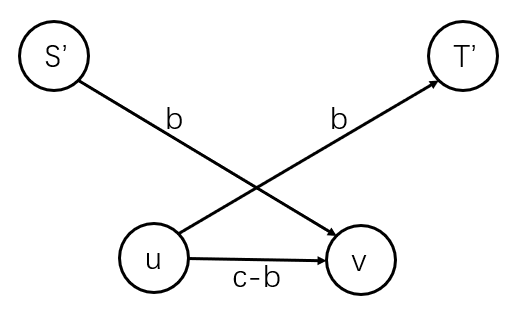
\includegraphics[scale = 0.5]{../src/graph/上下界网络流.png}

然后从$S'$到$S$, 从$T$到$T'$分别连容量为正无穷的边即可.

\textbf{有源汇上下界最小流}

按照上面的方法转换后先跑一遍最大流, 然后撤掉超级源汇, 反过来跑一次最大流退流, 最大流减去退掉的流量就是最小流.

\textbf{无源汇上下界可行流}

转化方法和上面的图是一样的, 只不过不需要考虑原有的源汇了.

在新图跑一遍最大流之后检查一遍辅助边, 如果有辅助边没满流则无解, 否则把每条边的流量加上$b$就是一组可行方案.

\subsubsection{常见建图方法}


\subsubsection{例题}
